\documentclass{article}
\usepackage{graphicx} % Required for inserting images
\usepackage{float}    % For the [H] float placement
\usepackage{amsmath}  % For math symbols like \text, \beta, etc.

\title{Econometrics - HW3}
\author{Felipe Manzi}
\date{October 2025}

\begin{document}

\maketitle

\section{resolution}

\textbf{Question 3 } 

\subsection*{(a) Draw the acceptance and rejection regions for this test using $\alpha = 5\%$.}

\begin{figure}[H]
  \centering
  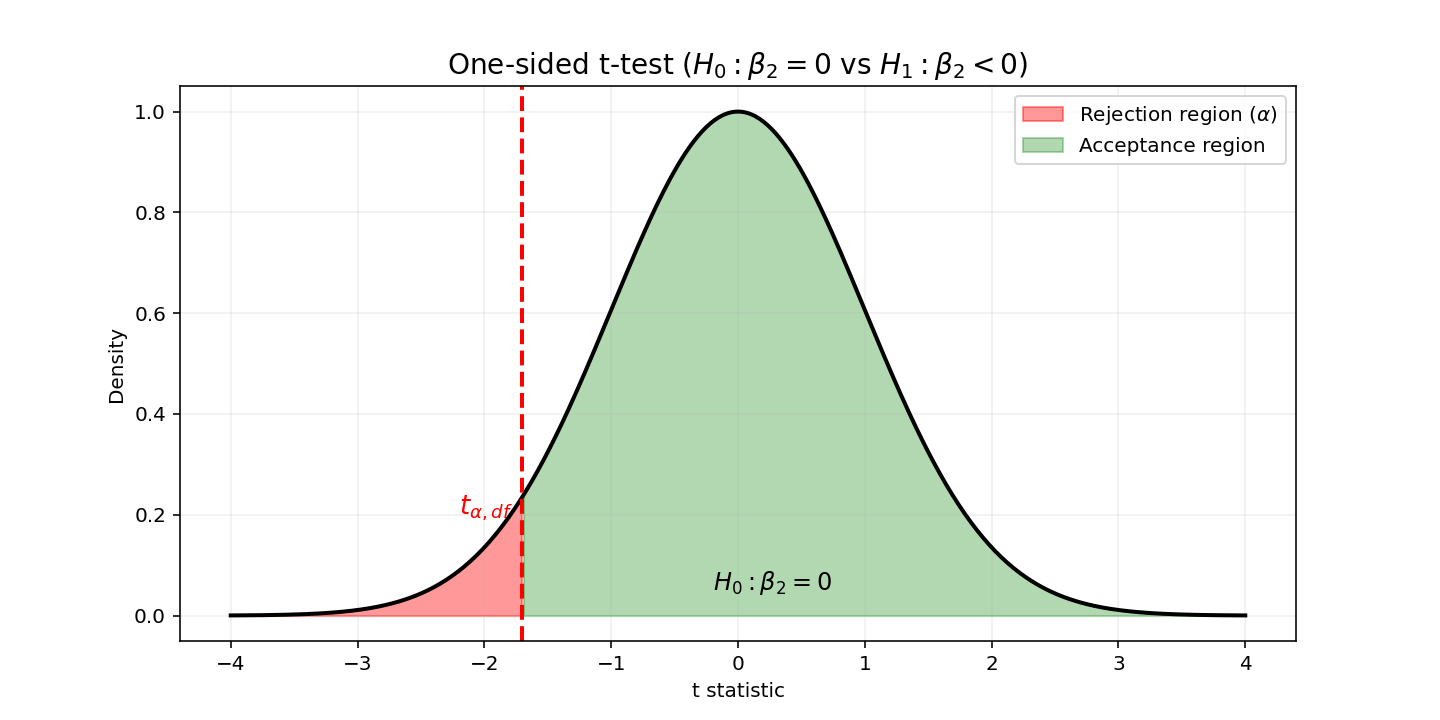
\includegraphics[width=0.9\linewidth]{example_critical_region.png}
  \caption{One-sided $t$-test with left-tail rejection region at level $\alpha$.}
\end{figure}

\subsection*{(b) Explain the intuition behind the location of the critical region.}

We test $H_0:\ \beta_2 = 0$ against the left--tailed alternative 
$H_1:\ \beta_2 < 0$ using the statistic
\[
t = \frac{\widehat{\beta}_2 - 0}{\mathrm{SE}(\widehat{\beta}_2)}.
\]
Under $H_0$, the statistic follows a Student-$t$ distribution centered at zero,
so most realizations of $t$ will lie near zero, with large positive or negative
values being unlikely.

This left-tail area has probability $\alpha$ under $H_0$ (in the example, $5\%$),
meaning that such extreme negative values of $t$ would occur only $5\%$ of the
time if $H_0$ were true. Observing one of these extreme outcomes provides
evidence that $\beta_2 < 0$, consistent with the alternative hypothesis, where we should reject $H_0$.

\textbf{Question 4 } 
\subsection*{(4.a) }

For any observation i:
\[
\begin{aligned}
y_i &= 10 + 5x_{2i} + u_i, \quad i = 1, \dots, 50. \\[6pt]
x_{2i} &\sim \text{Uniform}(0,\,20), \\[6pt]
u_i &\sim \mathcal{N}(0,\,6^2), \\[6pt]
\end{aligned}
\]

\subsection*{(4.b)}

\begin{enumerate}[(i)]

\item
The code generates \( M = 100 \) samples (or replications) of the regression model. 
Each sample contains \( n = 50 \) observations of the variables \( (y_i, x_{2i}) \).

\item All samples are generated from the same Data Generating Process (DGP):
\[
y_i = 10 + 5x_{2i} + u_i, \quad u_i \sim \mathcal{N}(0,6^2),
\]
with \(x_{2i} \sim \text{Uniform}(0,20)\).
That is, the true parameters \((\beta_1,\beta_2) = (10,5)\) and the error variance 
remain the same across replications. The only difference between samples arises 
from the random draws of the disturbance term \(u_i\).


\item:
The first part of the code initializes the simulation. 
The command \texttt{np.random.seed(1010)} fixes the random number generator to 
ensure that the simulation is fully replicable. The number of replications is set to 
\(M = 100\), and two arrays (\texttt{lower} and \texttt{upper}) are created to store the lower and 
upper bounds of the 95\% confidence intervals for each replication. 

Next, the explanatory variable is generated as 
\[
x_{2i} \sim \text{Uniform}(0,20), \quad i = 1, \dots, 50,
\]
and this vector is kept fixed across all replications. 
Then, for each simulation \(m = 1, \dots, 100\), a new sample of the dependent variable is generated as
\[
y_i^{(m)} = 10 + 5x_{2i} + u_i^{(m)}, \quad u_i^{(m)} \sim \mathcal{N}(0,6^2),
\]
which corresponds to repeated samples drawn from the same DGP with parameters 
\(\beta_1 = 10\), \(\beta_2 = 5\), and \(\sigma = 6\).

In each iteration, the code estimates by OLS the model, estimated slope, variance and standard error, and computes the 95\% 
confidence interval. Finally, these lower and upper bounds are stored in the matrix 
\texttt{CIs}, which contains one confidence interval per simulated sample.

\end{enumerate}

\subsection*{(4.c)}
The next part of the code evaluates the coverage performance of the constructed 
confidence intervals. Recall that the true value of the slope coefficient in the DGP is 
\(\beta_2 = 5\). Each interval stored in the matrix \texttt{CIs} has a lower bound 
\(\texttt{lower}[i]\) and an upper bound \(\texttt{upper}[i]\).

The command
\[
\texttt{IDg = np.where((lower <= 5) \& (upper >= 5))[0]}
\]
selects the indices of all samples whose 95\% confidence interval contains the true 
parameter value \(\beta_2 = 5\). In other words, it identifies the replications for which the 
interval estimate successfully covers the true slope. The number of such ``good'' intervals 
is stored in \texttt{length\_IDg}.

Conversely,
\[
\texttt{IDb = np.where(\textasciitilde((lower <= 5) \& (upper >= 5)))[0]}
\]
captures the indices of the ``bad'' intervals that fail to include the true value of 
\(\beta_2\). Their count is stored in \texttt{length\_IDb}.

Finally, the command
\[
\texttt{ratiog = (length\_IDg / M) * 100}
\]
computes the empirical coverage rate of the confidence intervals, expressed as a 
percentage. Since the theoretical confidence level is 95\%, the value of 
\texttt{ratiog} should be close to 95 if the finite-sample performance of the OLS-based 
intervals is consistent with their nominal level.


\subsection*{(4.d)}
The last part of the code produces a graphical representation of the $100$ confidence 
intervals constructed in the simulation. The horizontal axis corresponds to the parameter 
value $\beta_2$, while the vertical axis enumerates the simulated samples from $1$ to $100$. 
The command
\[
\texttt{plt.axvline(x=5, color='black', linestyle='--')}
\]
draws a vertical dashed line at the true value $\beta_2 = 5$, which serves as a reference 
point to evaluate whether each interval covers the true parameter.

Each horizontal line plotted representing the confidence interval obtained from simulation $j$, extending from its lower 
to upper bound. The color of each line depends on whether the corresponding interval 
contains the true value:
\begin{itemize}
    \item {\textbf{Gray}} intervals (\texttt{colors = 'gray'}) indicate that 
    the true $\beta_2 = 5$ lies within the estimated confidence bounds.
    \item {\textbf{Red}} intervals correspond to cases in which the true value 
    is not covered, i.e., the interval lies entirely above or below the dashed line.
\end{itemize}

By setting \texttt{xlim([4,6])} and \texttt{ylim([0,100])}, the plot zooms in on the relevant 
range of values for $\beta_2$ and displays the $100$ simulated intervals stacked vertically. 

\subsection*{(4.e)LETS THINK ON THIS ONE BEFORE SENDING NOT SURE IF SHOULD SEND THIS ENTIRE}

\begin{figure}[H]
  \centering
  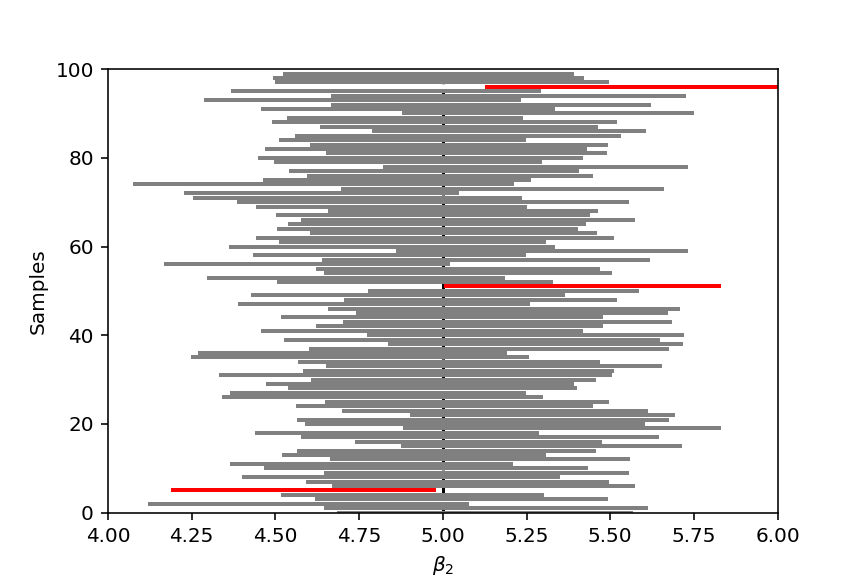
\includegraphics[width=0.9\linewidth]{imagem_exercise.png}
  \caption{Simulation with 100 samples of IC intervals }
\end{figure}

The empirical coverage rate obtained was \(0.92\) (or \(92\%\)), which is not 
particularly surprising given that the simulation included only \(M = 100\) replications. 
Because the coverage indicator in each replication is a Bernoulli variable with 
probability \(p = 0.95\), the estimated coverage rate will naturally fluctuate due to 
Monte Carlo sampling variation. With a limited number of replications, these fluctuations 
can be noticeable, and obtaining a value slightly below \(0.95\) is entirely expected. 

\subsection*{(4.f)}

This graphical representation provides an intuitive visualization of the concept 
of \emph{confidence level}: under repeated sampling, approximately $95\%$ of the 
intervals constructed using the $t$-distribution formula are expected to contain 
the true parameter. In this particular simulation, about $92\%$ of the intervals 
cross the dashed line, which aligns with the empirical coverage rate computed 
earlier and illustrates the inherent sampling variability when the number of 
replications is finite, in this case "small".

\subsection*{(4.g LETS THINK IF NEED THIS COMPLEXITY OR JUST THE INTUITON)}

Let $I_m=\mathbf{1}\{\text{CI}_m \text{ contains } \beta_2\}$ be the indicator of
coverage in replication $m$ and let $p=\Pr(I_m=1)$. In our setting (normal,
homoskedastic errors; fixed $x$), the usual $t$–interval for $\beta_2$ has
\emph{exact} $95\%$ finite–sample coverage conditional on $x$, hence $p=0.95$.
The reported statistic is
\[
\texttt{ratiog} \;=\; \frac{1}{M}\sum_{m=1}^M I_m,
\]
the sample mean of i.i.d.\ Bernoulli$(p)$ variables. Therefore,
\[
\mathbb{E}[\texttt{ratiog}]=p=0.95,\qquad
\operatorname{Var}(\texttt{ratiog})=\frac{p(1-p)}{M}.
\]
By the Law of Large Numbers, $\texttt{ratiog}\xrightarrow{a.s.} p$ as $M\to\infty$;
by the CLT,
\[
\sqrt{M}\,(\texttt{ratiog}-p)\;\xrightarrow{d}\; \mathcal{N}\!\left(0,\;p(1-p)\right).
\]
Hence increasing $M$ from $100$ to $10{,}000$ leaves the \emph{expected} value at
$0.95$ but reduces the standard error from
$\sqrt{0.95\cdot0.05/100}\approx 0.0218$ (2.18 p.p.) to
$\sqrt{0.95\cdot0.05/10{,}000}\approx 0.00218$ (0.218 p.p.). Consequently a
95\% normal approximation interval for the empirical coverage shrinks from
$[0.906,\,0.994]$ at $M{=}100$ to $[0.946,\,0.954]$ at $M{=}10{,}000$. Thus we
should expect \texttt{ratiog} to be much closer to $95\%$ with $M{=}10{,}000$,
which matches the large–$M$ run (about $94.9\%$).

\subsection*{(4.h) Changing the quantile to build 99\% CIs ALSO WORTH LOOKING HERE}

Replacing $0.975$ by $0.995$ in the $t$ quantile produces a \emph{99\%} confidence
interval for $\beta_2$:
\[
\left[\;\widehat\beta_2 - t_{0.995,\nu}\,\mathrm{SE}(\widehat\beta_2),\;
       \widehat\beta_2 + t_{0.995,\nu}\,\mathrm{SE}(\widehat\beta_2)\;\right],
\qquad \nu = n-2 = 48 .
\]
Under the classical linear model with normal, homoskedastic errors and fixed $x$,
this $t$–interval has \emph{exact} finite–sample coverage $p=0.99$ (conditional on $x$).
With $M=10{,}000$ replications, the reported statistic
\[
\texttt{Ratio}=\frac{1}{M}\sum_{m=1}^{M}\mathbf{1}\{\text{CI}_m\ \text{contains}\ \beta_2\}
\]
is the sample mean of i.i.d.\ Bernoulli$(p)$ variables, so
\[
\mathbb{E}[\texttt{Ratio}]=0.99,\qquad
\mathrm{SE}(\texttt{Ratio})=\sqrt{\frac{p(1-p)}{M}}
=\sqrt{\frac{0.99\cdot0.01}{10{,}000}}\approx 0.0010 .
\]
By the CLT, a 95\% normal approximation interval for the empirical coverage is
\[
0.99 \pm 1.96\times 0.0010 \approx [0.988,\;0.992].
\]
Hence we would expect \texttt{Ratio} to be very close to $99\%$ (within about $\pm0.2$ percentage points).

\paragraph{Effect on the plot.}
Because $t_{0.995,\nu}>t_{0.975,\nu}$, the intervals become \emph{wider} (both endpoints move farther from
$\widehat\beta_2$). Consequently, almost all intervals (about $99\%$) cross the vertical line at the true value
$\beta_2=5$; only about $1\%$ fail to cover. Visually: many fewer “non-covering” intervals and uniformly wider
segments.

\subsection*{(4.i) Purpose of the simulation}

This exercise illustrates:
\begin{itemize}
  \item the meaning of a confidence interval as a \emph{procedure with coverage}: across repeated samples,
        a $1-\alpha$ CI contains the true parameter with probability $1-\alpha$ (here verified empirically by \texttt{Ratio});
  \item how the nominal level ($95\%$ vs.\ $99\%$) trades off \emph{coverage} and \emph{width} (higher coverage $\Rightarrow$ wider CIs);
  \item in the classical normal homoskedastic regression with fixed regressors, the $t$–interval achieves
        its \emph{exact} nominal coverage in finite samples, which the simulation confirms as $M$ becomes large.
\end{itemize}


\end{document}
